\newcommand{\degree}{\ensuremath{^{\circ}}}

\chapter{Kreslenie molekuly}

Po tom čo získame a aplikujeme mapovanie medzi šablonovou a cieľovou molekulou RNA,
získame cieľovú molekulu s čiastočnou vizualizáciou, ktorej zvyšok potrebujeme dopočitať.

Príklad ako to vyzerá je na obrázku \ref{obr:frog_to_human}, kde sme
namapovali sekundárnu štruktúru malej podjednotky rRNA 23S žaby (X04025) do
obrázka sekundárnej štruktúry malej podjednotky rRNA 23S človeka.
Ako si môžeme všimnúť, v obrázku (najmä v spodnej časti) sú bázy nakreslené
sivo - tie sa chystáme zmazať. V obrázku nám tak vzniknú prázdne miesta.
Naopak po insertoch potrebujeme vypočítať, kam umiestníme daný pár,
resp. samotnú bázu, prípadne pre ňu musíme urobiť miesto a posunúť zvyšok
molekuly. Update vrcholu nerobí žiadne štruktúrne zmeny, zmení sa iba
báza na danom mieste.

\begin{figure}
  \centering
  %trim=left bottom right top
  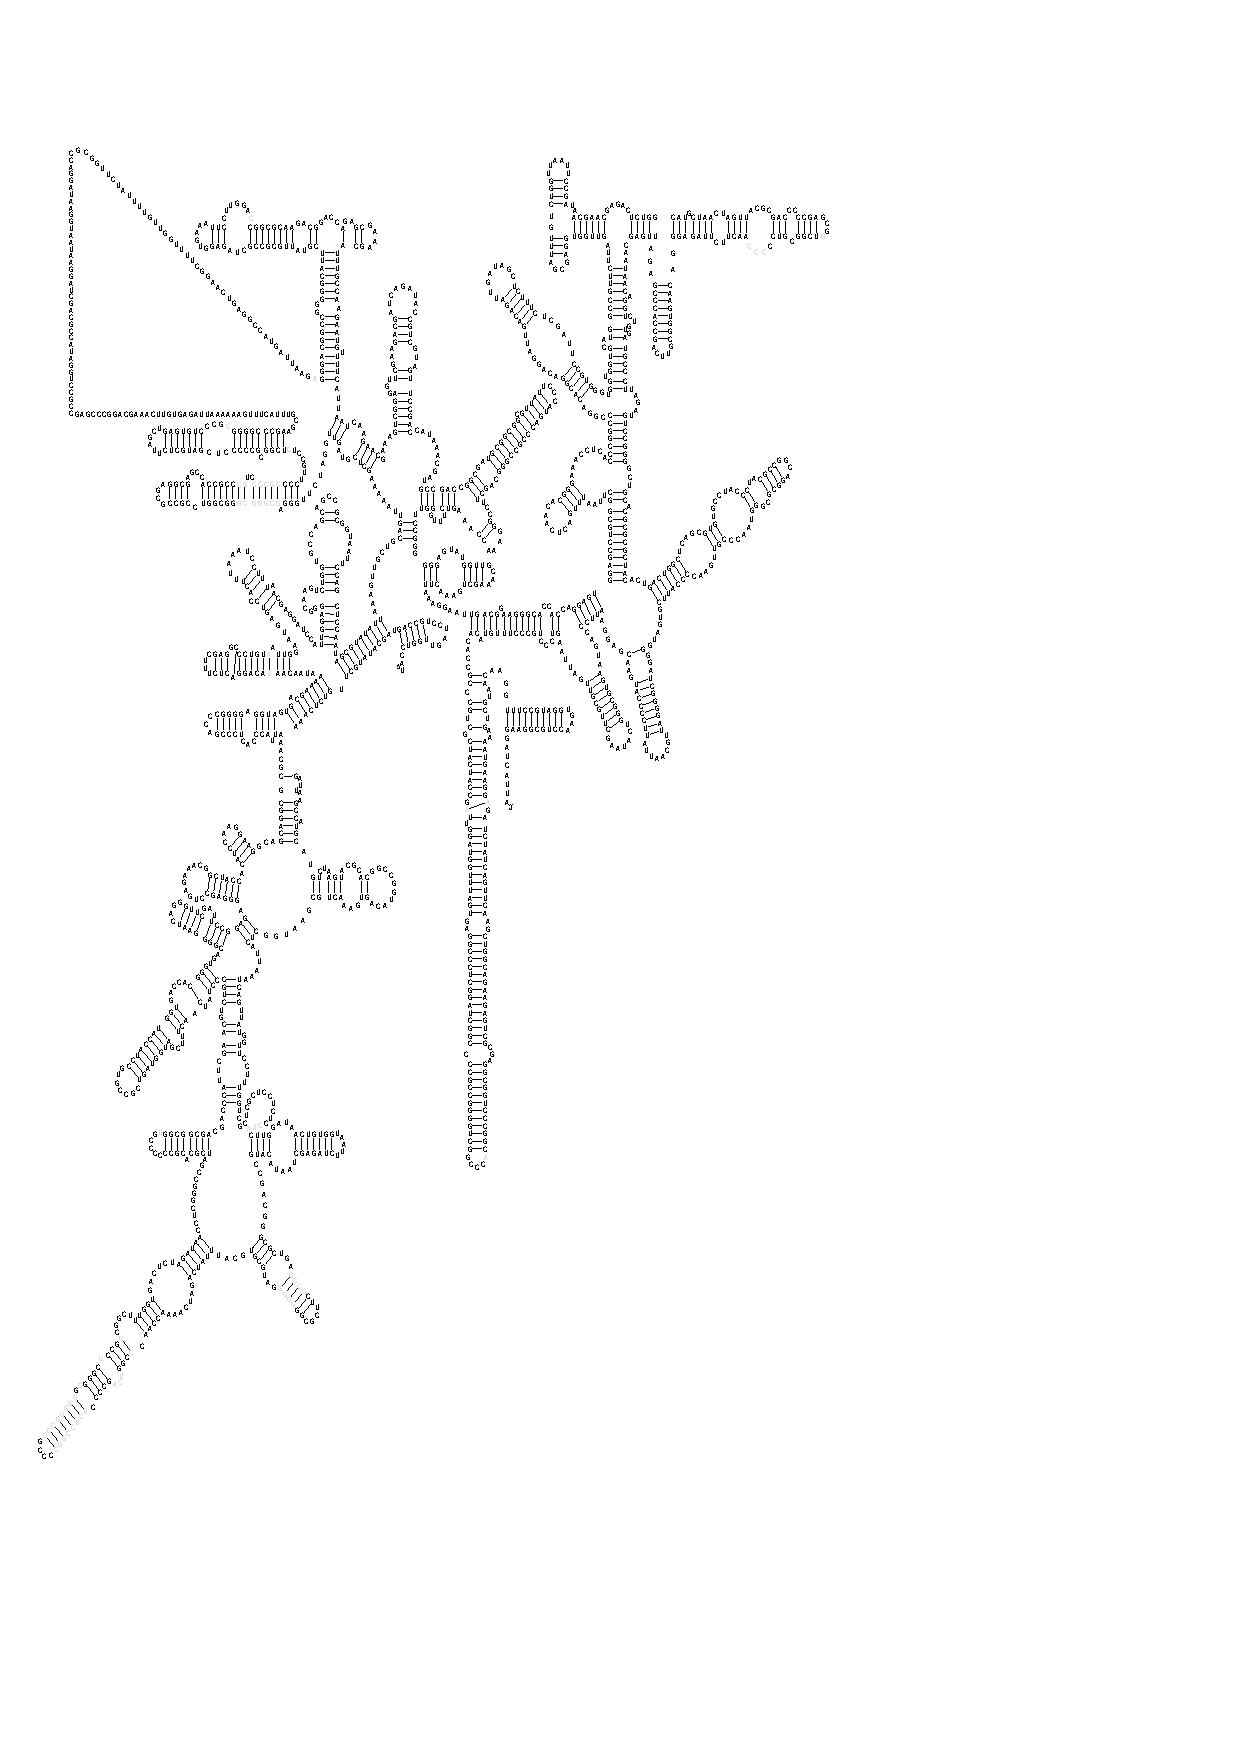
\includegraphics[clip, trim=0 5cm 6cm 2cm, width=1\textwidth]{../img/african_frog-to-human-mapped}
  \caption{Namapovanie rRNA žaby do obrázka rRNA človeka z \ref{obr:human_crw}, sivou sú označené mazané bázy}
  \label{obr:frog_to_human}
\end{figure}

Čiastočnej vizualizácie sa chceme dotýkať čo najmenej. To znamená, že všetky zásahy sa
snažíme robiť iba v miestach, ktoré sa zmenili - boli dotknuté vkladaním alebo mazaním báz.

Jediné dve výnimky budú normalizácia vzdialeností medzi bázovými pármi a vyrovnávanie stemov.





\section{Normalizácia vzdialeností v bázových pároch a vyrovnavanie stemov}

Tieto dve výnimky sme sa rozhodli urobiť, keďže časté výnimky nám sťažovali
prácu a veci, ktoré predpokladáme, že v obrázku nájdeme neboli vždy skutočnosťou.

Ako príklad môžeme uviesť, že ak chceme nakresliť nový bázový pár a máme nakreslený
rodičovský párový vrchol. Následne v smere od jeho rodiča (nášho prapredka) kreslíme nový
bázový pár. Tu môže nastať chyba, ktorú ilustrujeme na obrázku \ref{obr:insert_stem_error}.

\begin{figure}[H]
  \centering
  %trim=left bottom right top
  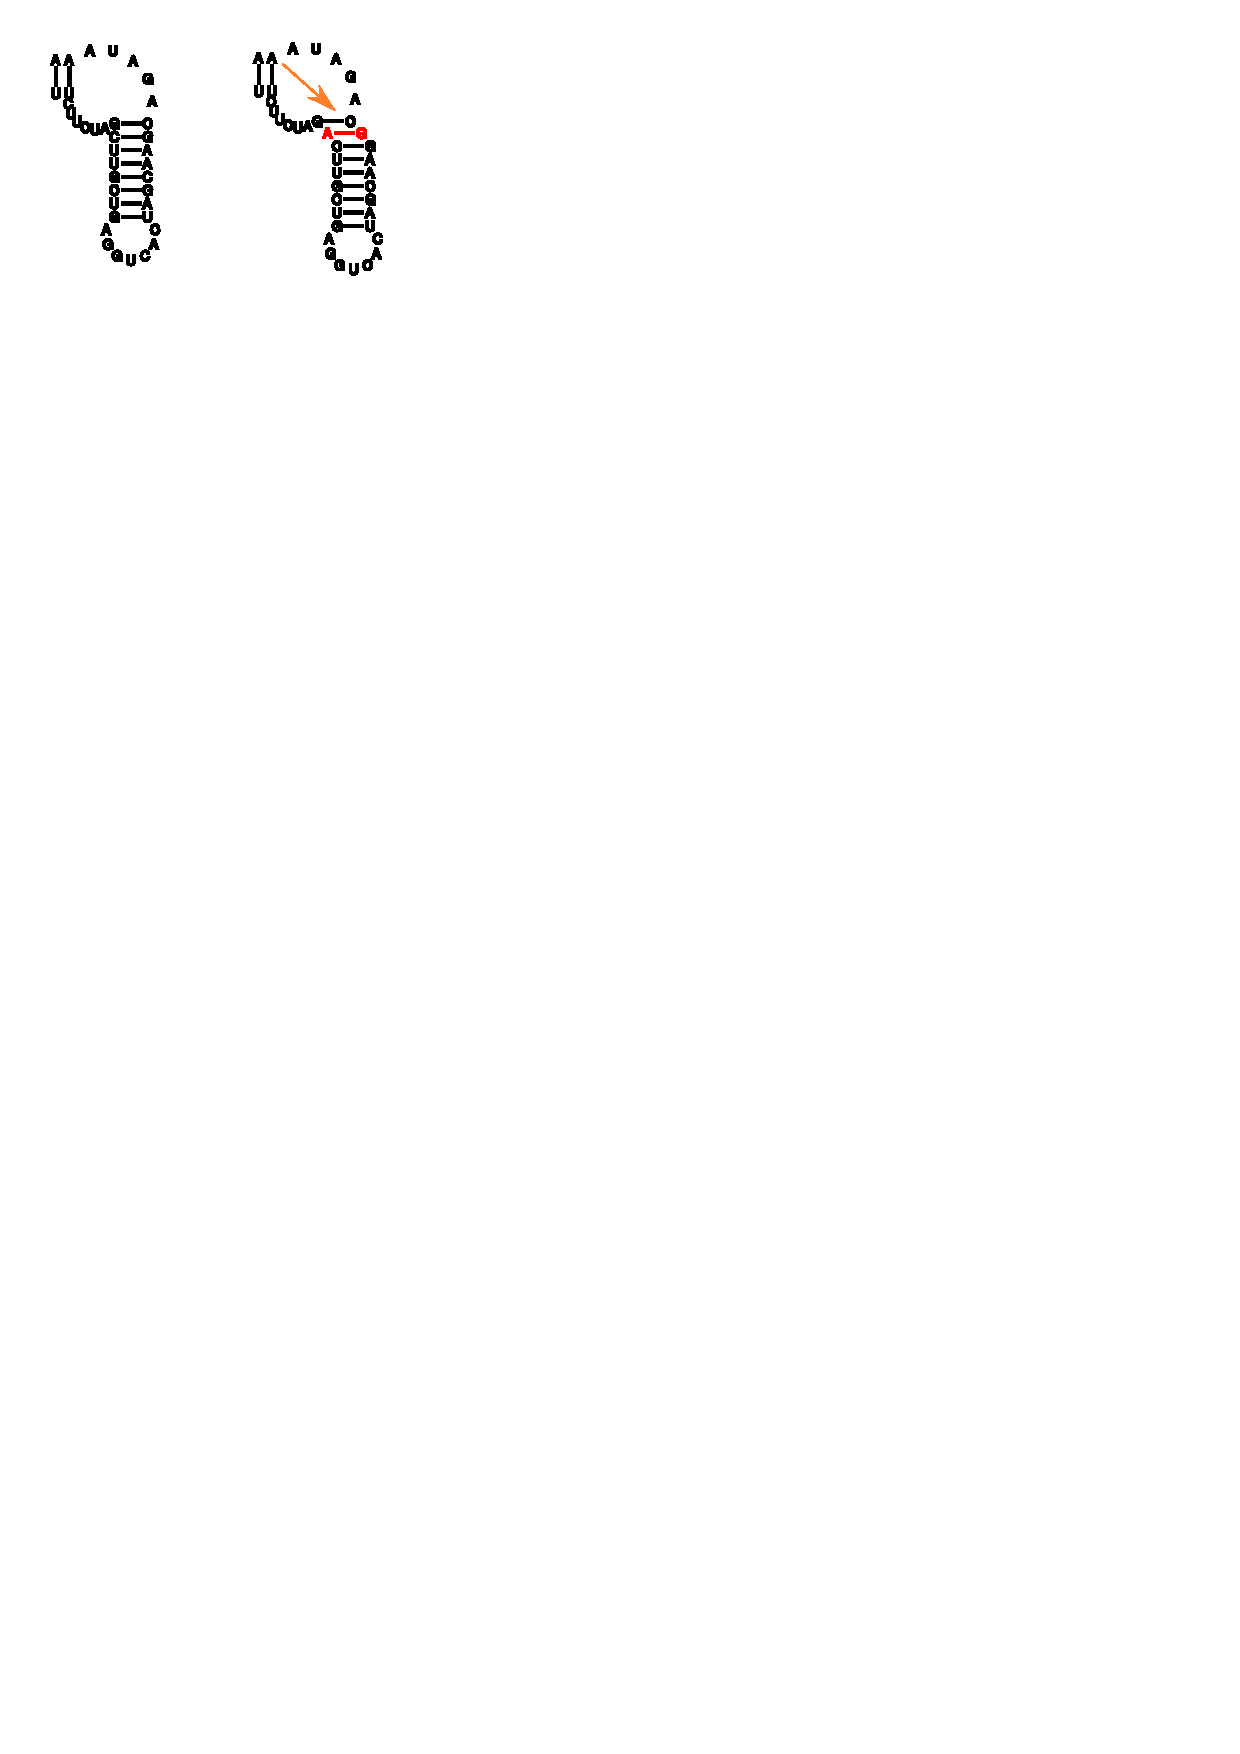
\includegraphics[clip, trim=0 24.5cm 14cm 0]{../img/alg/even_stem/error_insert}
  \caption{Možná chyba pri vkladaní nového bázového páru}
  \label{obr:insert_stem_error}
\end{figure}

Vyrovnávací algoritmus prejde všetky stemy a z ich začiatkov vedie priamku na ktorej
majú podľa pravidla byť uložené všetky stemové vrcholy. Následnými rotáciami
a posunutiami podstromov ich uložíme na miesto.




\section{Operácie na stromoch}

Čitateľa zoznámime s 2 operáciami, ktoré budeme vykonávať na molekule. Tie využijeme
ako pri vkladaní, tak aj pri mazaní vrcholov zo stromu.

\begin{algorithm}
  \caption{Rozloženie báz po kružnici}
  \label{alg:operacia_circle_reinsert}
  \begin{algorithmic}[1]
    \Procedure {RozlozBazy}{$Begin, End, Bases$}
      \State $n \gets$ $Bases.size()$
      \State $\Gamma \gets$ kružnica pre $n$ bodov prechádzajúca bodmi $Begin$ a $End$
      \State $\Pi \gets$ rozdel kruhový oblúk kružnice $\Gamma$ od $Begin$ po $End$ na $n$ bodov
      \ForAll{$i$ in $1 \dots n$}
        \State nastav pozíciu bázy $Bases[i]$ na $\Pi[i]$
      \EndFor
    \EndProcedure
  \end{algorithmic}
\end{algorithm}

\begin{algorithm}
  \caption{Posunutie podstromu}
  \label{alg:operacia_tree_shift}
  \begin{algorithmic}[1]
    \Procedure {PosunPodstrom}{$Root, Vector$}
      \ForAll {vrchol $V$ v podstrome vrcholu $Root$}
        \If {vrchol $V$ už má určenu pozíciu v obrázku - nieje práve vložený}
          \State pripočítaj k pozicií bázy $V$ vektor $Vector$
        \EndIf
      \EndFor
    \EndProcedure
  \end{algorithmic}
\end{algorithm}

Ako sme písali už skôr, všetky loop štruktúry majú byť uložené na kružniciach.
K tomu nám pomôže funkcia \ref{alg:operacia_circle_reinsert}.
Tá dostáva na vstupe zoznam báz $Bases$ a dva body v rovine, $Begin$ a $End$.
Týmito bodmi potrebujeme viesť kružnicu, ktorá bude dostatočne veľká, aby
na ňu všetky bázy zo zoznamu vošli. Veľkosťou kružnice v tomto prípade myslíme
dĺžku jej kruhového oblúku medzi vrcholmi $Begin$ a $End$.

V našom programe používame iteračný algoritmus. Ten začne s kružnicou so stredom
medzi $Begin$ a $End$ bodmi a pomaly ju zväčšuje alebo zmenšuje.
Nakoniec buď nájde kružnicu, ktorej veľkosť je optimálna, alebo ani na maximálny
počet krokov takú kružnicu nenájde a tak vráti tú z posledného kroku.
To sa môže stať napríklad, ak je samotná vzdialenosť medzi bodmi príliš veľká.

Na obrázku \ref{obr:insert_circle_hairpin} vidíme celý algoritmus zväčšovania kružnice.
Začíname kružnicou medzi $Begin$ a $Eend$ bodmi, ktoré reprezentujú bázy posledného
páru v smere $5' \to 3'$. V ďalších dvoch iteráciách zväčšujeme kružnicu až kým
nieje dostatočne veľká pre daný počet báz. Následne vrcholy hairpinu
na ňu uložíme.
Pôvodné vrcholy sú označené modrou, vložené sú zase červené I.

\renewcommand{\wi}{0.24\textwidth}

\begin{figure}
  \begin{subfigure}{\wi}
%trim=left bottom right top
    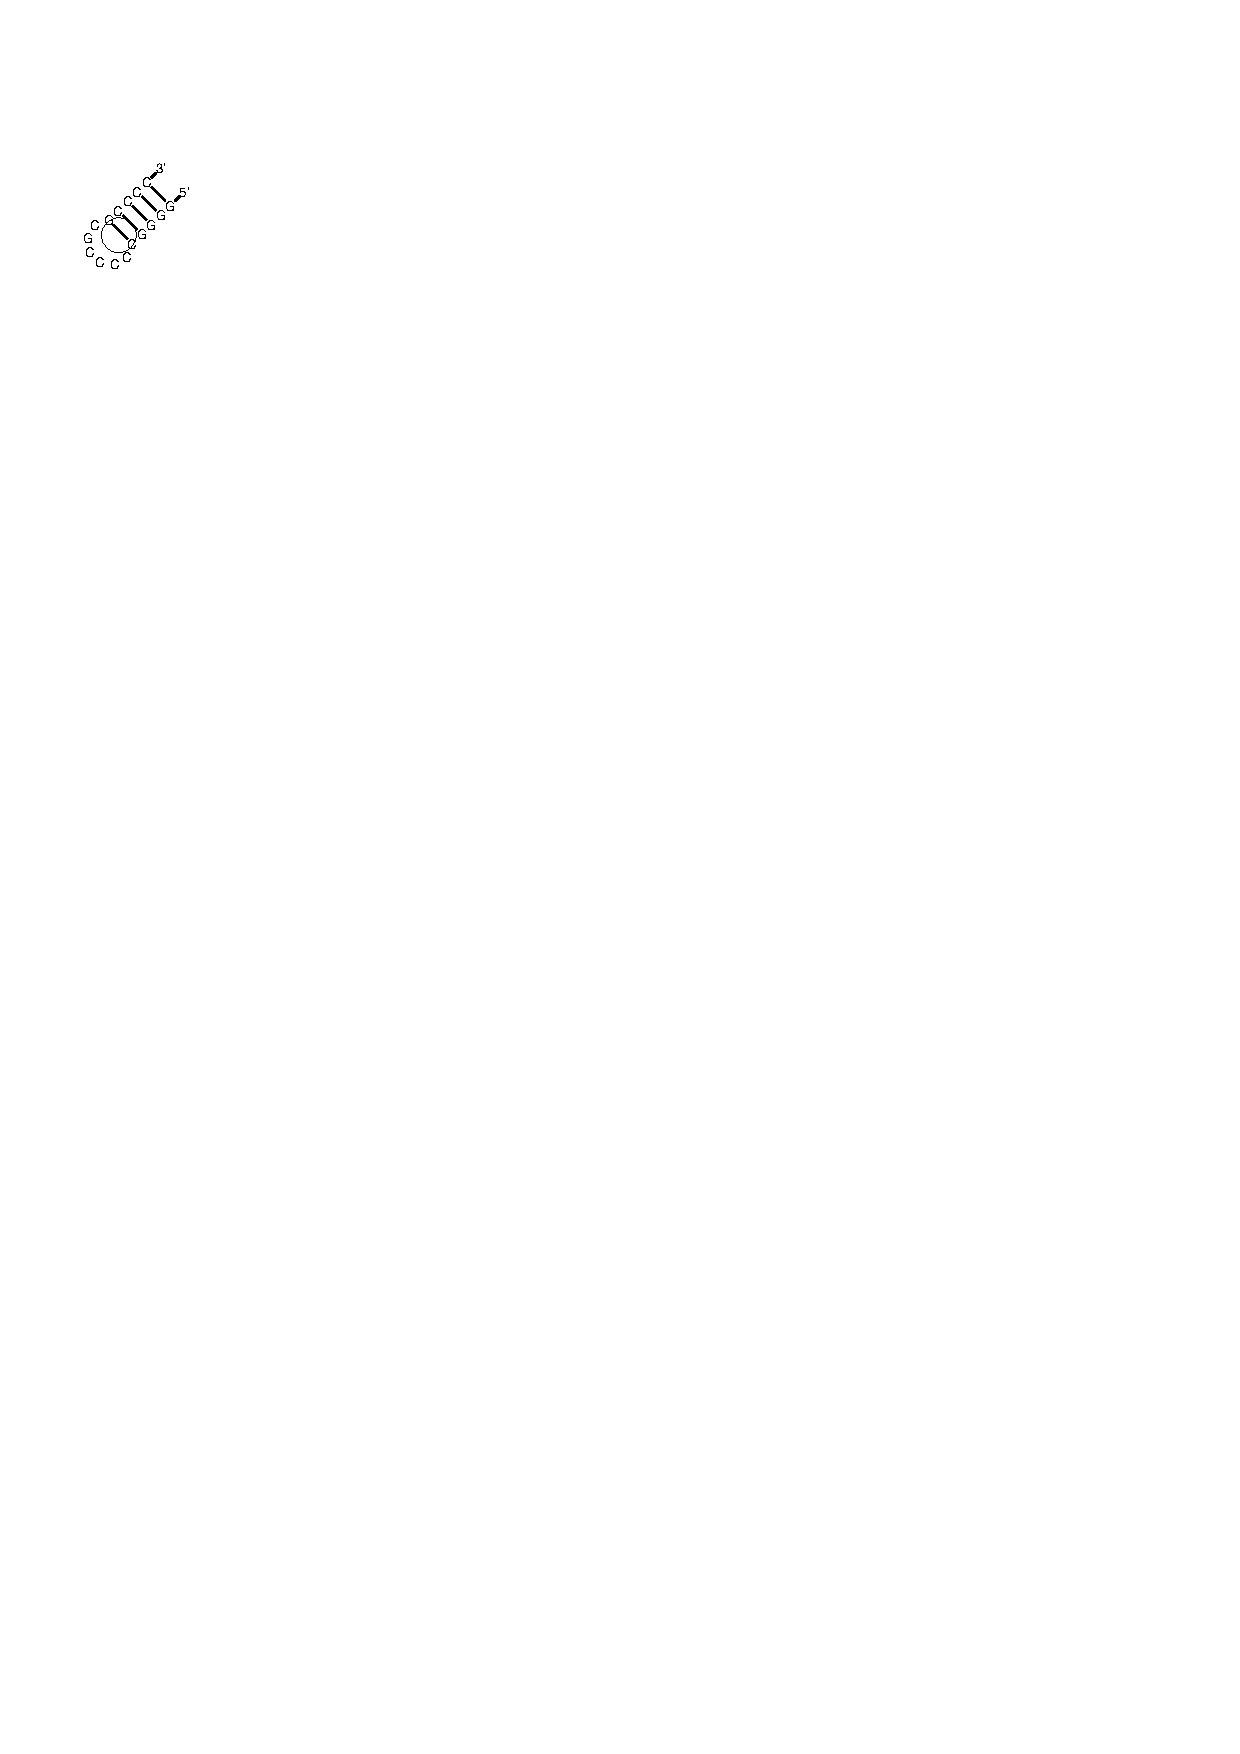
\includegraphics[trim=1cm 24.5cm 17.5cm 2.5cm]{../img/alg/insert/1/circle-small-begin}
  \end{subfigure}
  \begin{subfigure}{\wi}
    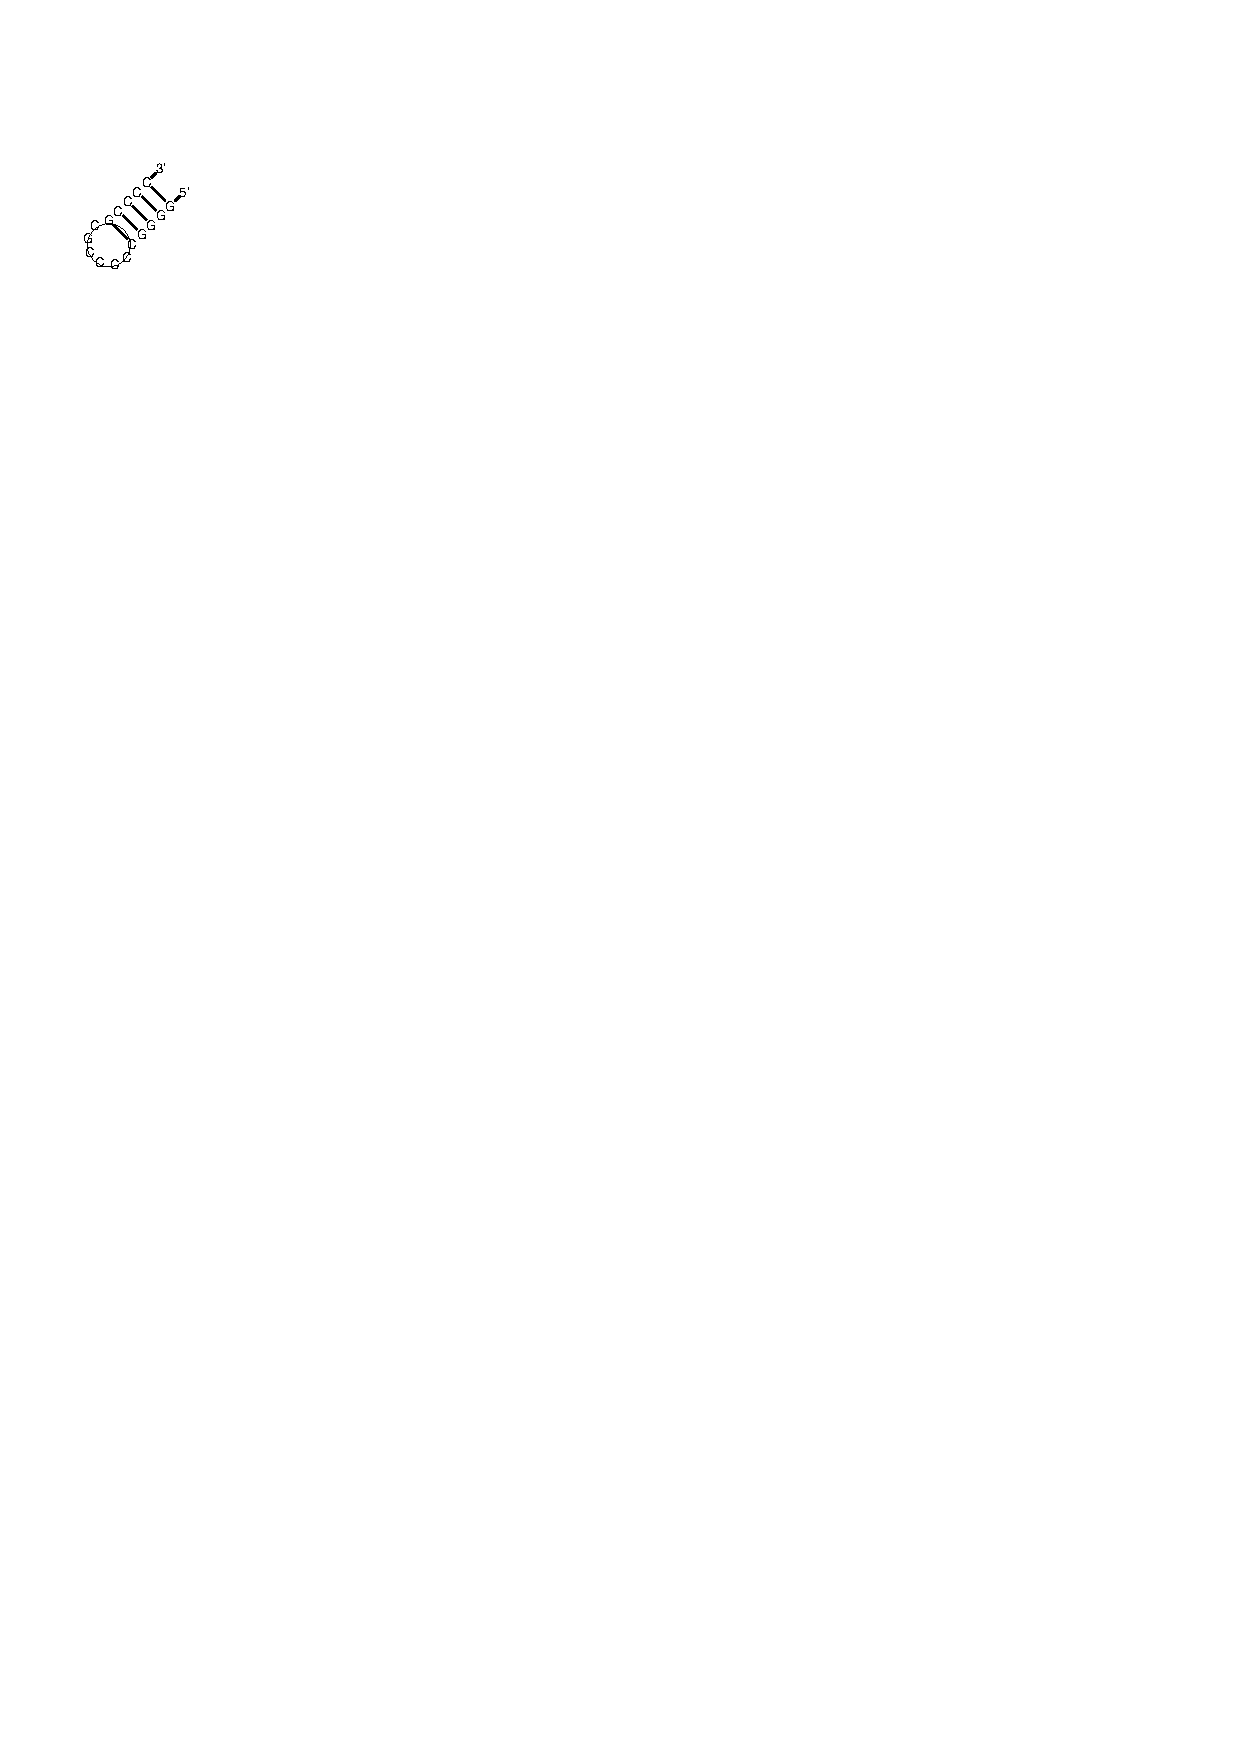
\includegraphics[trim=1cm 24.5cm 17.5cm 2.5cm]{../img/alg/insert/1/circle-small}
  \end{subfigure}
  \begin{subfigure}{\wi}
    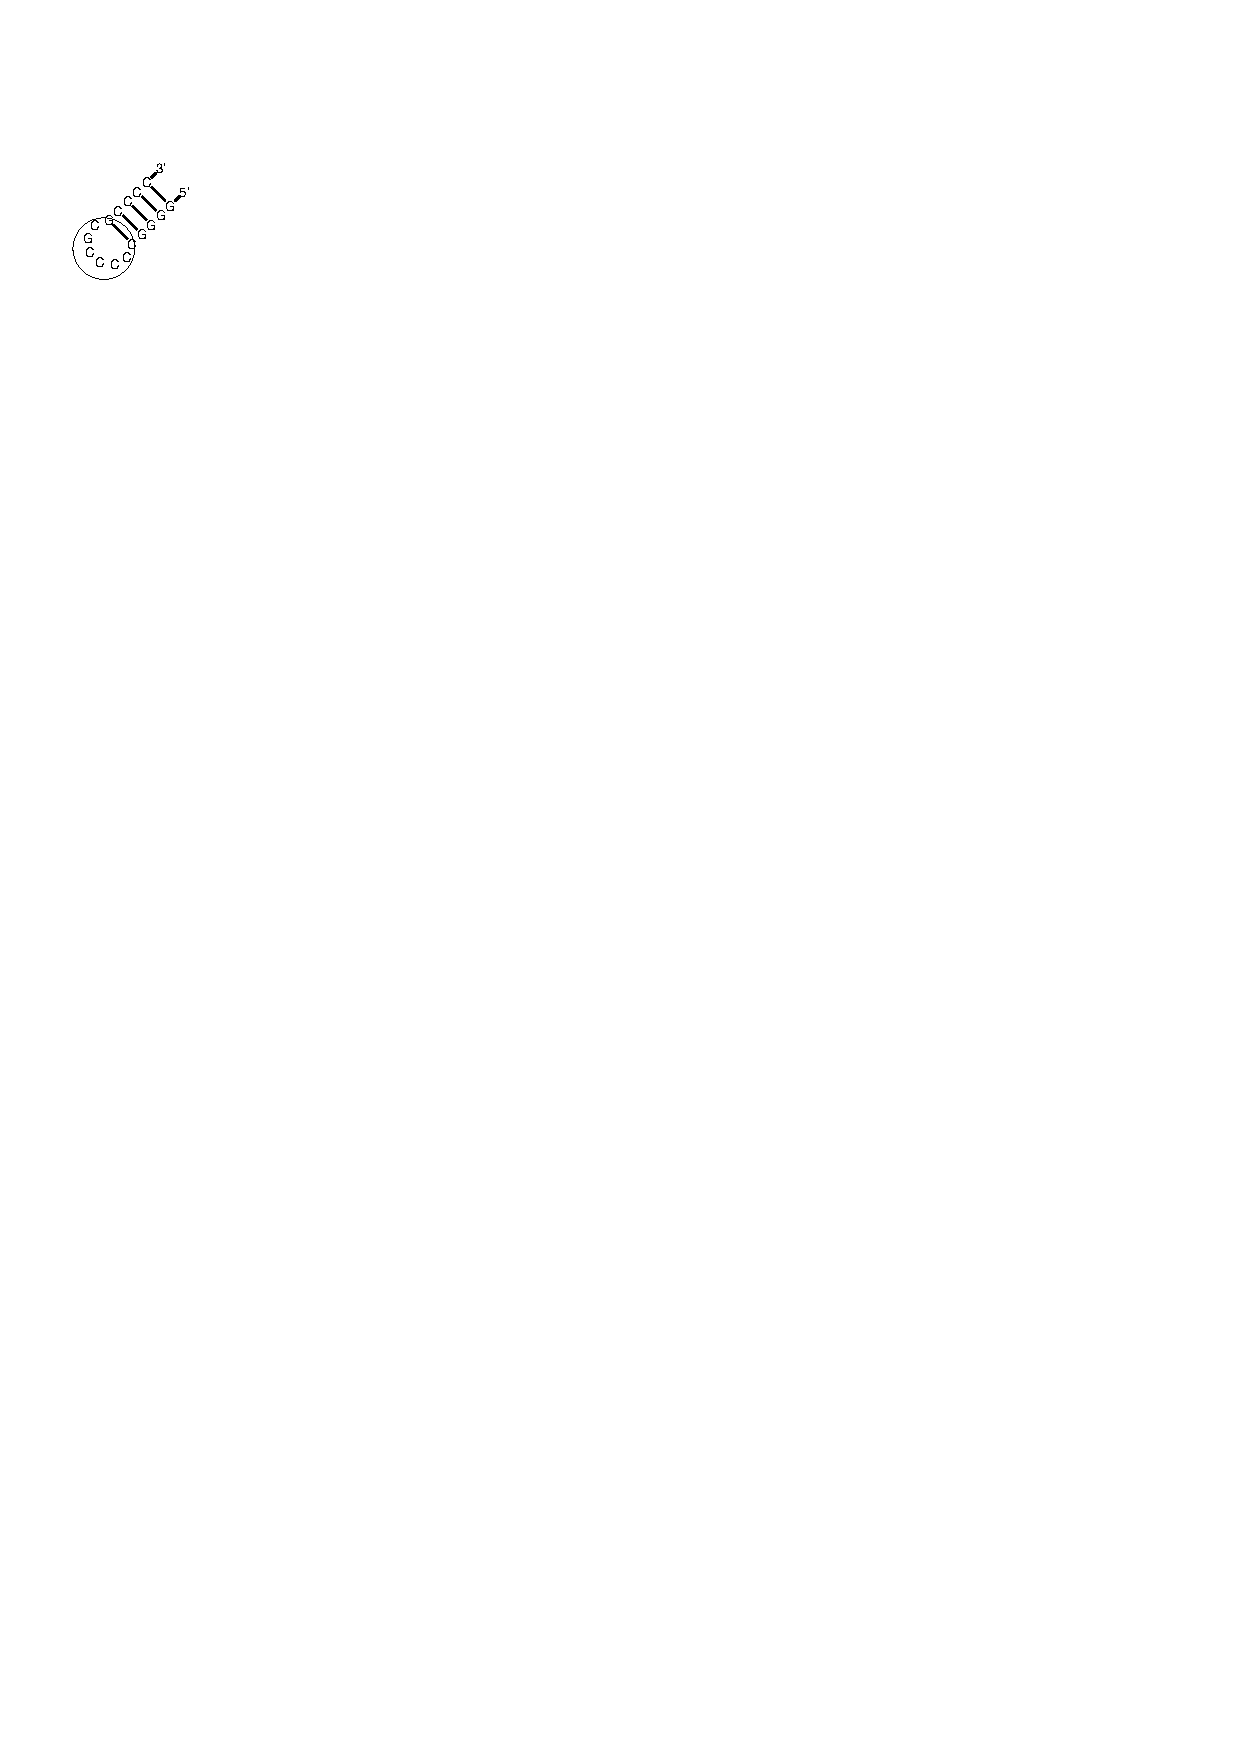
\includegraphics[trim=1cm 24.5cm 17.5cm 2.5cm]{../img/alg/insert/1/circle-big}
  \end{subfigure}
  \begin{subfigure}{\wi}
    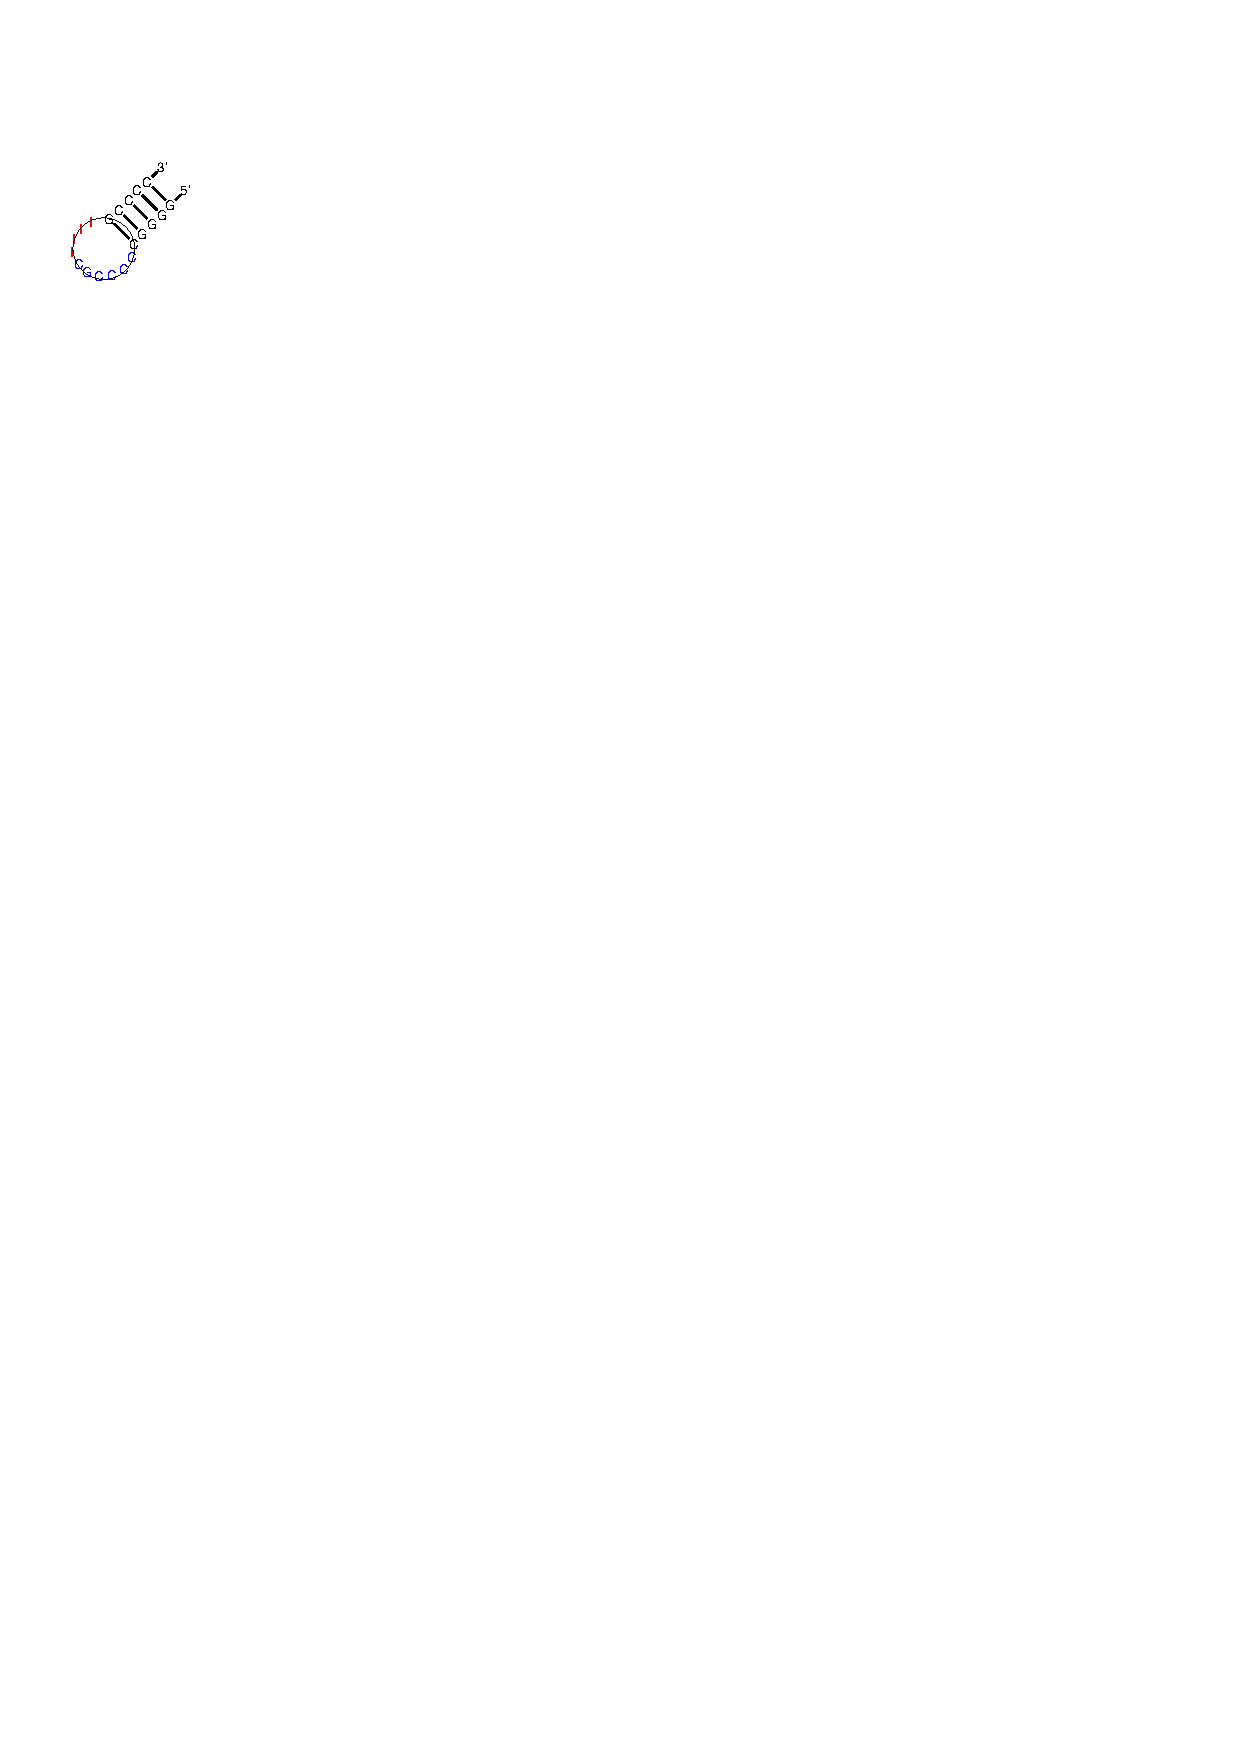
\includegraphics[trim=1cm 24.5cm 17.5cm 2.5cm]{../img/alg/insert/1/circle-big-end}
  \end{subfigure}

  \caption{Príklad zväčšovania kružnice a následne vloženie báz}
  \label{obr:insert_circle_hairpin}
\end{figure}





\subsection{Vkladanie nového vrcholu do stromu}

Pri vkladaní nového vrcholu do stromu môžu nastať nasledovné možnosti.

Ak vkladáme listy do hairpinu, je to jednoduché. Potrebujeme iba použiť
procedúru z algoritmu \ref{alg:operacia_circle_reinsert}
s parametrami $Begin = $ požicia prvej bázy z bázového páru, $End = $ pozícia
druhej bázy z páru a $Bases = $ zoznam všetkých potomkov.
Príklad sme už ukázali na obrázku \ref{obr:insert_circle_hairpin}.

Trochu zložitejšie je to pri vkladaní listu do stemu. V tomto prípade buď už stem
obsahoval nejaký loop, alebo musíme vytvoriť novú. Potrebujeme upraviť vzdialenosť
medzi vrcholmi stemu, teda posunuť celý podstrom tak, aby nám tu všetky bázy vošli.
To vyriešime algoritmom \ref{alg:operacia_tree_shift}. Následne postupujeme
rovnako ako pri vkladaní nukleotidu do hairpinu - nájdeme kružnicu a bázy
na ňu naukladáme.

Vloženie bázového páru do stemu je jednoduché. Najprv posunieme celý podstrom
a tým urobíme miesto pre novú dvojicu báz. Následne ich uložíme na pozíciu kam patria.
Názorný príklad vkladania je na obrázku \ref{obr:insert_stem}.
Môže sa stať, že zdedíme niekoľko nepárových báz z predka. V tom prípade iba
znovu prekreslíme tieto loopy.


\renewcommand{\wi}{0.45\textwidth}

\begin{figure}
  \centering
  \begin{subfigure}{\wi}
%trim=left bottom right top
    \includegraphics[clip, trim=1cm 25cm 14cm 1cm, width=1\textwidth]{../img/alg/insert/stem}
    \caption{Vkladanie bázových párov}
  \end{subfigure}
  \begin{subfigure}{\wi}
%trim=left bottom right top
    \includegraphics[clip, trim=8cm 25cm 7cm 1cm, width=1\textwidth]{../img/alg/insert/stem}
    \caption{Vytvorenie novej loopy v steme}
  \end{subfigure}
  \caption{Vkladanie báz do stemu}
  \label{obr:insert_stem}
\end{figure}




\subsection{Modifikácia multibrach loop}

Modifikácia multibranch loop je zložitejšia ako všetky predchádzajúce prípady.
Obrázky sú väčšinou ručné upravené tak, aby bol čo najkompaktnejší a kvôli tomu
sa často nerešpektujú všetky pravidlá, napríklad kružnicový tvar štruktúry.

Kvôli tomu sa snažíme do tejto štruktúry nezasahovať, ak je to možné.
Vyhnúť sa tomu môžeme napríklad pri malej zmene počtu listov medzi jednotlivými vetvami.
Ak je dostatočne malá, môžeme sa pokúsiť vrcholy roztiahnúť od seba, alebo naopak ich
priblížiť k sebe a tak viac využiť miesto medzi vetvami. Tento prípad je znázorneny
na obrázku \ref{obr:insert_multibranch}.

Naopak, ak sa jedná o pridanie, alebo odobratie celej vetvy, modifikácií sa nevyhneme.
V tom prípade rozdistribuujeme vrcholy z loopy (spolu so spárovanými bázami tvoriacimi
vetvy) na kružnicu. Je to podobný proces, ako používame iba pre samotné loopy,
ale potrebujeme ešte zrotovať vetvy do správneho smeru a po prípade ich aj zrotovať.






\subsection{Mazanie vrcholov zo stromu}

Mazanie považujeme za inverznú operáciu ku vkladaniu a vzhľadom k použitým operáciám
sa od neho vôbec nelíši - ak sme urobili zásah do stemu či loopu, prekreslíme
ich rovnako ako to bolo v prípade vkladania báz.




